\section{Elektronik}\label{sec:elektronik}
%\textbf{Sicherheitshinweis:} Vorsicht beim Umgang mit den Chemikalien und immer eine Schutzbrille tragen.
\subsection{Ansteuerung}
In diesem Kapitel werden verschiedene Arten und Möglichkeiten der Ansteuerung des LCD diskutiert.

\subsubsection{Spannungsart}
Das LCD Display sollte mit einer Rechteck-Wechselspannung angesteuert werden. Gleichspannung würde die Flüssigkristalle auf Dauer unwiederherstellbar elektrolytisch zersetzen und den Display somit unbrauchbar machen.

\subsubsection{Spannungshöhe}\label{subsec:spannung}
Es gibt zwei ausschlaggebende Kriterien:
\begin{itemize}
\item Minimalste Spannung, so dass noch ein gut sichtbares Bild erscheint
\item Spannung, bei der ein möglichst geringer Strom fließt\\
\end{itemize}

Unter einer Rechteck-Wechselspannung von -2\,V - +2\,V wird die Anzeige zu schwach, um klar etwas erkennen zu können. Mit steigender Spannung nimmt nur die Schnelligkeit zu, mit der das Anzeigefeld angezeigt wird, die Intensität nimmt nicht weiter zu. Ab einer Spannung von 6V besteht die Gefahr, dass auch benachbarte Felder aufleuchten. So wurde bei unserem Testdesign (Abbildung \ref{testmuster}) \textit{Darth Vader} auf Platte 1 und die \textit{kleinen Rechtecken} auf Platte 2 angeschlossen. Die \textit{kleinen Rechtecken} wurden angezeigt.

Die Stromstärken wurden mit einem Multimeter gemessen. Im Ruhezustand hat das Messgerät bereits einen Strom von -2\,$\mu$A 
 angezeigt. Wir bewegen uns im Mikroamperebereich weshalb die folgenden Messwerte nur als Richtwerte zu verstehen sind. Sie spiegeln aber sehr gut wieder, dass ein LCD sehr energiesparend ist.

\begin{table}[]
	\centering
	\caption{Stromfluss bei verschiedenen Spannungswerten und Anzeigen}
	\label{my-label}
	\begin{tabular}{p{1.2cm}|p{1.2cm}|p{1.2cm}|p{1.2cm}|p{1.2cm}}
		DC Spannung & großes Rechteck (\(22,5\times22,5\,\textrm{mm}\)) & kleine Rechtecke (\(10\times10\,\textrm{mm}\)) & Darth Vader & Walter White    \\
        {[}V{]} & {[}$\mu$A{]} & {[}$\mu$A{]} & {[}$\mu$A{]} & {[}$\mu$A{]} \\
         \hline
		10 & 0,47 & -- & --  & --   \\ \hline
		5  & 0,27 & 0,12 & 150 & 0,02 \\ \hline
		4  & 0,23 & 0,08 & 66  & 0,04 \\ \hline
		3  & 0,18 & 0,07 & 37  & 0,03 \\ \hline
		2  & 0,13 & 0,06 & 9   & 0,04 \\
	\end{tabular}
	\label{tab:volt}
\end{table}

Tabelle \ref{tab:volt} zeigt die Messungen der Stromstärken in Mikroampere der einzelnen Testanzeigedesigns bei einer angelegten Gleichspannung. Dies ist für einen Dauerbetrieb nicht zu empfehlen (siehe Abschnitt \ref{subsec:spannung}), wurde aber zur Vereinfachung der Messung so gewählt. Weshalb die Anzeige von “Darth Vader” so hohe Stromstärken aufweist ist noch unklar.

\subsubsection{Frequenz}
Zur Feststellung mit welcher Frequenz das LCD angesteuert werden sollte, haben wir eine Rechteckspannung mit unterschiedlichen Frequenzen an verschiedenen Elektroden angelegt. Unter einer Frequenz von 30\,Hz fängt die Anzeige an zu flackern, da das menschliche Auge dort das Umschalten feststellen kann. Über einer Frequenz von 1\,MHz lässt die Intensität merklich nach. Um den Mikrocontroller stromsparend benutzen zu können, sollte aber eine möglichst geringe Frequenz verwendet werden.

\subsubsection{Ansteuerungsart}
Da für eine Einzelansteuerung jedes einzelnen Symbols zu viele Mikrocontrollerausgänge benötigt werden, wird auf das Multiplexverfahren zurückgegriffen. Dieses spielt vor allem bei einer Symbolbelegung von \(4\times4\) Symbolen auf einer Glasplatte aus.

%Bisher wurden die Glasplatten nur einzeln angesteuert. Dadurch wären bei einem \(2\times4\) Aufbau 8 Anschlüsse an jeder Glasplatten nötig. Will man mehrere Symbole, z.B. \(4\times4\) anschließen, wären pro Glasplatte 16 Anschlüsse von Nöten. Um den Aufwand zu verringern, stehen 2 Möglichkeiten zur Verfügung: 
%Zum einen kann auf die Glasplatte 1 die Elektrodenstruktur aufgebracht werden und jede Elektrode einzeln verbunden werden. Auf Glasplatte 2 muss dann nur eine gemeinsame Fläche für alle Anzeigesymbole angebracht werden, da nur die Symbole an der Stelle aufleuchten, an der beide Glasplatten angesteuert werden. Eine weitere Möglichkeit ist die Ansteuerung per Multiplexverfahren. Hierbei müssen z.B. bei einer \(4\times4\) Platte nur 4 Anschlüsse pro Platte angebracht werden. Das verschafft mehr Platz für die Anschlüsse an der Glasplatte und die Fehlerwahrscheinlichkeit von schlechter Kontaktierung wird verringert. Außerdem kann dadurch ein kleinerer Mikrocontroller eingesetzt werden, da weniger Ausgangspins benötigt werden. Dadurch steigen jedoch die Anforderungen an die Software. Wie die Platten dann an den Mikrokontroller angeschlossen werden steht im Abschnitt \ref{subsec:platine}.\\

%Aufgrund der oben genannten Vorteile des Multiplexverfahrens haben wir dieses für die Ausarbeitung unseres Displays genutzt. Seine Vorteile spielt es vor allem bei einer Symbolbelegung von \(4\times4\) Symbolen auf einer Glasplatte aus.\\

Zur Ansteuerung des LCD wird idealerweise eine Rechteckspannung von \(-3\,\textrm{V}\) bis \(3\,\textrm{V}\) bei einer Frequenz von \(50\,\textrm{Hz}\) im Mulitplexverfahren verwendet.

%Zusammenfassend sind also folgende Ansteuerparameter optimal für die Ansteuerung dieses LCD:
%\begin{itemize}
%\item Rechteckspannung von \(-3\,\textrm{V}\) bis \(3\,\textrm{V}\)
%\item Frequenz \(50\,\textrm{Hz}\)
%\item Multiplexverfahren\\
%\end{itemize}

\subsection{Spannungsversorgung}
Als Spannungsversorgung könnten somit 2 Standard Batterien mit je \(1,5\,\textrm{V}\) verwendet werden. Diese sinken durch Entladung auf eine Mindestspannung von \(0,9\,\textrm{V}\) ab. Dadurch wird die Anzeige nicht bis zur vollen Entladung der Batterien halten. Je nach Wahl des Mikrocontroller kommt dieser auch nicht mit \(1,8\,\textrm{V}\) Spannung aus. Deshalb haben wir uns entschieden drei Batterien mit je \(1,5\,\textrm{V}\) einzusetzen.

\subsection{Anbindung}
Um das LCD Display mit der Ansteuerplatine zu verbinden gibt es mehrere Möglichkeiten. Da nur ein sehr geringer Strom (\(\mu A\)) fließt und eine Spannung von \(3\,\textrm{V}\) angelegt wird ist nur eine dünne Drahtzuleitung (\(0,5\, mm^2\)) von Nöten. Im folgenden werden verschiedene Verfahren diskutiert mit denen eine Anbindung möglich ist.

\subsubsection{Klemmen}
Im ersten Test wurde das Display über Klemmen angesteuert. Dies hat einwandfrei funktioniert, jedoch beschädigen die Klemmen die Glasplatten und stellen somit keine gute Endlösung dar.

\subsubsection{Conductive Paint}
\cite[\textit{Conductive Paint}]{conductivepaint} ist eine schwarze leitfähige Farbe die von der Firma bareconductive hergestellt wird. Die Flüssigkeit kommt aus der Tube und braucht circa 15 Minuten zum Trocknen. Jedoch ist die Festigkeit zu schwach und kann die Drähte nicht fest an den Glasplatten fixieren. Deshalb muss noch eine zusätzliche Schicht Kleber (2-Komponentenkleber, Sekundenkleber) darüber angebracht werden, um die Festigkeit zu steigern.

\subsubsection{Kupferfolie}
Kupferfolie wäre eine weitere Idee, die allerdings noch nicht getestet wurde.

\subsection{Platine}\label{subsec:platine}

\subsubsection{Anforderungen}
Die Platine (Schaltplan siehe Abbildung \ref{shematic}) dienst zur Ansteuerung des LCD und soll es ermöglichen, die Uhr zu stellen und die richtige Uhrzeit anzuzeigen. Es soll die Möglichkeit geben das Display nicht nur im BCD Format zu betreiben, sondern auch in anderen Formaten, wie zum Beispiel rein binär.

\subsubsection{Wahl des Mikrocontrollers}
Der Mikrocontroller muss mindestens zwei Eingänge für zwei Taster zur Uhrzeitstellung zur Verfügung stellen. Des Weiteren werden 4 weitere Pins für den Anschluss der ISP Schnittstelle zum Programmieren des Mikrocontrollers benötigt. Je nach Anzahl der anzuzeigenden Symbole und ob das Multiplexverfahren verwendet wird oder nicht,  sind noch zusätzliche Ausgänge nötig. Wenn man den Mikrocontroller der Atmel-Reihe verwendet, ist des Weiteren auf die Endbezeichnung P zu achten, da der Mikrocontroller dann stromsparender ist. Außerdem muss der Versorgungsspannungsbereich in dem von der Batterie zur Verfügung gestelltem Bereich liegen. Deshalb wurde für dieses Projekt der \cite[ATmega88PA]{atmel88pa} gewählt.

\subsubsection{Wahl der Bauteile}
Um die Uhrzeit so exakt wie möglich zu erhalten, wurde eine spezieller 32,768\,kHz Quartz verwendet, der auf Uhrenandwendungen spezialisiert ist. Bis auf den Mikrocontroller und dem Quartz wurden nur SMD Bauteile verwendet, um die Platine zu einem späteren Zeitpunkt komplett auf SMD Bauteile umstellen zu können. Zum Entprellen der Taster wurde jeweils ein 100\,nF Kondensator parallel geschlossen. Der Eingang der Spannungsversorgung (VCC, AVCC) wurde ebenfalls mit je einem 100\,nF Kondensator versehen, um eine stabile Eingangsspannung zu gewährleisten. Der Pin Aref wurde über einen Kondensator mit 100\,nF auf Masse gezogen. Dieser Kontakt kann dazu genutzt werden, um den Batteriestand festzustellen. Für die SMD Bauteile wurde eine Größe von 0805 gewählt.

\subsubsection{Herstellung der Platine}

Das Platinenlayout (Abbildung \ref{board}) wurde mit der kostenlosen Version von Eagle erstellt. Anschließend wurde die komplette Platine im FAUFabLab gefertigt. Eine Anleitung hierzu befindet sich auf der Homepage des \cite[FAUFabLab]{fablabwerkzeuge}, weshalb hier nicht näher darauf eingegangen wird.

%\textbf{Sicherheitshinweis:} Vorsicht beim Umgang mit den Chemikalien und immer eine Schutzbrille tragen. Das Ätzbad kann Löcher in der Kleidung verursachen, weshalb es ratsam ist alte Kleidung zu tragen.\\


%Das Platinenlayout wurde mit der kostenlosen Version von Eagle erstellt. Die Platine wurde komplett im FAUFabLab geätzt und bestückt. Die Leiterbahndicke beträgt 16\,mil, der Abstand der Massefläche zu den Leiterbahnen beträgt ebenfalls 16\,mil. Die Bohrlochdurchmesser der Vias und Löcher zum aufstecken der Bauteile beträgt 0,9\,mm. Das Boardlayout wurde auf Papier im FAUFabLab ausgedruckt und auf die kupferbeschichtete Seite der Platine gelegt. Anschließend werden diese zusammen für 09:40\,min in den Belichter gelegt.  Wichtig ist, dass man die Platinen vor dem Belichten an den Rändern entgratet, um ein gutes Belichtungsergebnis zu erreichen. Zudem ist darauf zu Achten, dass die Schutzfolie auf der Kupferseite, die mit dem Fotolack beschichtet ist, abzunehmen. Anschließend kommt die Platine in den Entwickler (NaOH) bis sich der Fotolack an den Stellen, an denen er mit UV-Licht belichtete wurde, ablöst. Nachdem die Platine gut mit Wasser abgespült wurde, wird sie in das Ätzbad (Natriumpersulfatlösung) gelegt. Wenn sich die Kupferschicht zwischen den Leiterbahnen komplett abgelöst hat sollte die Platine entnommen werden. Belässt man sie zu lange im Ätzbad besteht die Gefahr, dass zusätzlich Leiterbahnen angeätzt werden. Anschließend die Platine gut mit Wasser abwaschen und für 1:30min in den Belichter legen. Dannach noch ein letztes mal entwickeln und gut abwaschen. Anschließend die Platine ins Verzinnungsbad (Bungard SurTin chemische Verzinnungslösung) geben, um die Kupferschicht vor Korrosion zu schützen. Nun können die Löcher bebohrt und die Platine bestückt werden.
%Wenn das Ätz- oder Verzinnungsbad zu alt ist kann dies zu schlechten Ergebnissen führen.\\
%Weitere Informationen zur Herstellung von Platinen und bis zu welcher Leiterbahndicke die Herstellung möglich ist gibt es auf der Homepage des \cite[FAUFabLab]{fablabwerkzeuge}.

\begin{figure}[t]
  \centering
  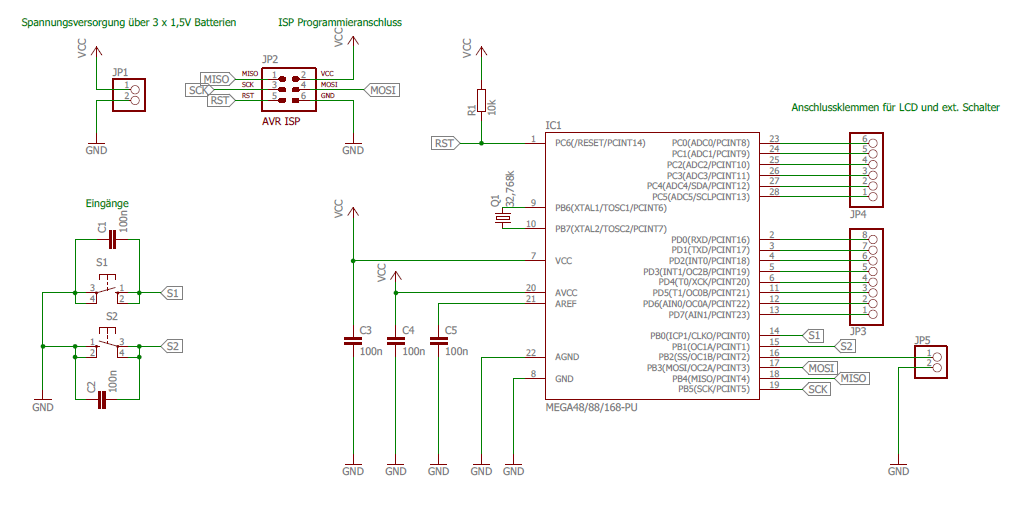
\includegraphics[width=1\linewidth, keepaspectratio]{Bilder/DIYShematic}
  \caption{Schaltplan (erstellt mit Eagle)}
  \label{shematic}
\end{figure}

\begin{figure}[t]
  \centering
  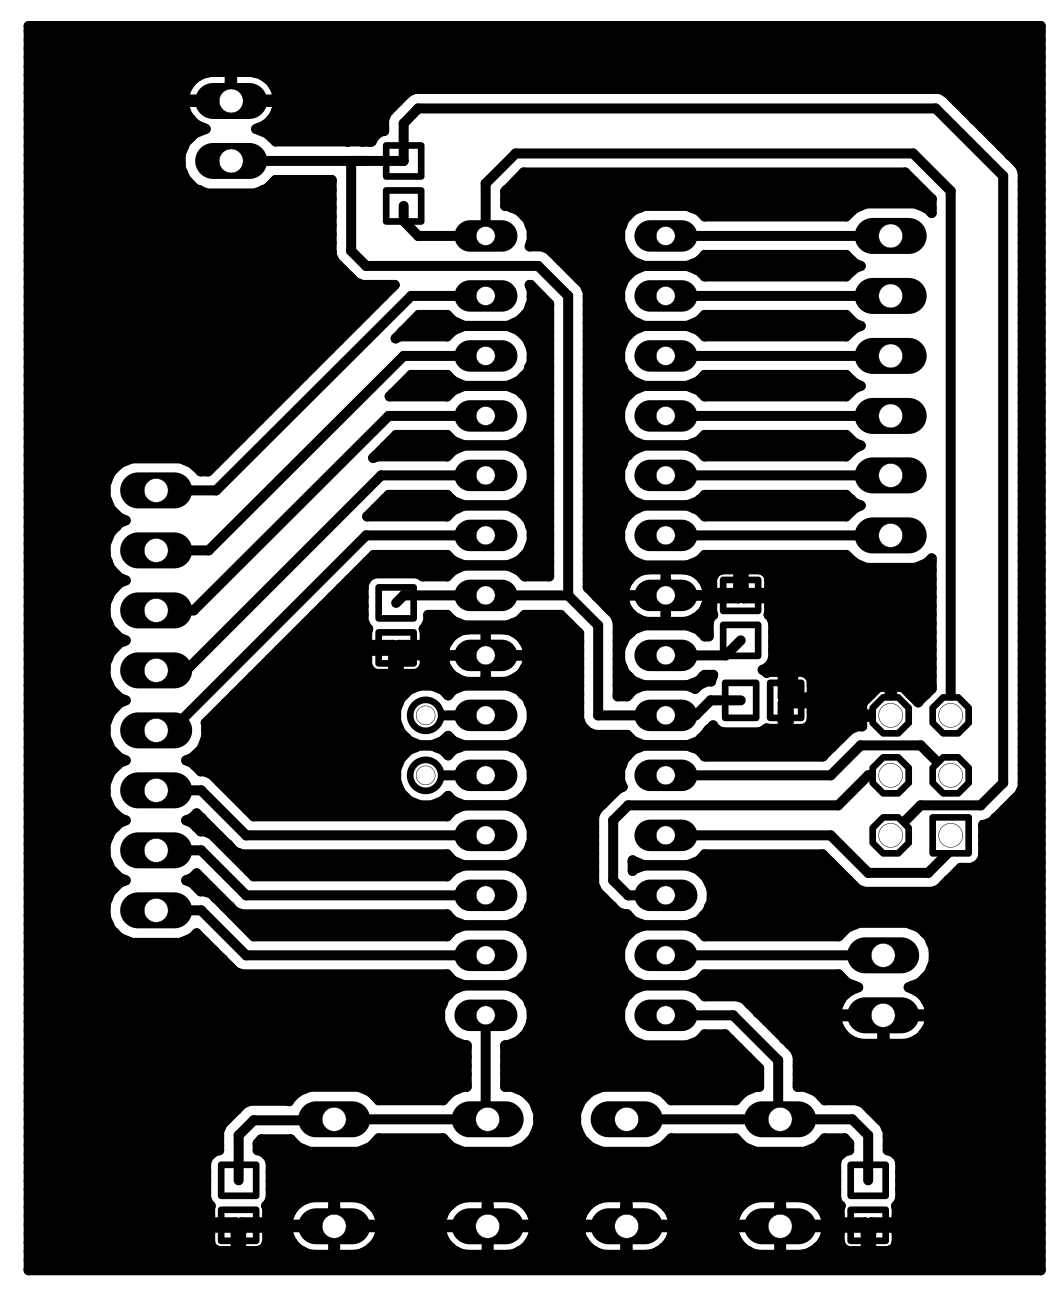
\includegraphics[angle=90, width=0.5\linewidth, keepaspectratio]{Bilder/DIYBoard}
  \caption{Platinenlayout (erstellt mit Eagle)}
  \label{board}
\end{figure}